\documentclass[10pt,letterpaper]{article}

\usepackage[utf8]{inputenc}
\usepackage[T1]{fontenc}
\usepackage{lmodern}
\usepackage[margin=0.45in,top=0.40in,bottom=0.40in]{geometry}
\usepackage{amsmath,amssymb,bm}
\usepackage{graphicx}
\usepackage{booktabs}
\usepackage{tabularx}
\usepackage{xcolor}
\usepackage{hyperref}
\usepackage[expansion=false]{microtype}
\usepackage{tcolorbox}
\usepackage{titlesec}
\usepackage{enumitem}

\graphicspath{{../figures/}{../../docs/engineering_reports/figures/}}

\definecolor{threevblue}{RGB}{15, 65, 130}
\definecolor{threevorange}{RGB}{220, 100, 20}
\definecolor{darkgray}{RGB}{35, 42, 54}
\definecolor{lightbg}{RGB}{246, 250, 254}
\definecolor{bordergray}{RGB}{210, 225, 240}

\hypersetup{
    colorlinks=true,
    linkcolor=threevblue,
    urlcolor=threevorange,
    citecolor=threevblue
}

\pagestyle{empty}

\titleformat{\section}{\large\bfseries\color{threevblue}}{}{0em}{}[\vspace{-0.4em}\rule{\linewidth}{0.8pt}\vspace{-0.3em}]

\tcbset{
    sharp corners,
    boxrule=0.8pt,
    colframe=threevblue,
    colback=lightbg,
    left=6pt,right=6pt,top=5pt,bottom=5pt
}

\begin{document}

% HEADER BOX
\begin{tcolorbox}[colframe=threevblue,colback=threevblue,coltext=white,boxrule=0pt,top=6pt,bottom=6pt]
\begin{minipage}[c]{0.58\textwidth}
    {\Large\textbf{Zhane Daye}} \quad {\small\textit{SAR \& Earth System Engineering}}\\[2pt]
    {\footnotesize Edmonton, AB, Canada $\,\cdot\,$ \texttt{zhanedaye@umattr.ca} $\,\cdot\,$ \href{https://www.linkedin.com/in/zhane-umattr}{linkedin.com/in/zhane-umattr}}
\end{minipage}
\hfill
\begin{minipage}[c]{0.40\textwidth}
    \raggedleft
    {\large\textbf{TARGET: 3v GEOMATICS}}\\[1pt]
    {\footnotesize\textbf{Role:} Senior InSAR Analyst / Scientific Computing Developer}\\[1pt]
    {\scriptsize Geotechnical Ground Displacement \& Mining Slope InSAR}
\end{minipage}
\end{tcolorbox}

\vspace{-4pt}

% SUB-BANNER QUICK LINKS
\begin{tcolorbox}[colframe=bordergray,colback=lightbg,top=3pt,bottom=3pt]
\footnotesize
\textbf{Live 3D Mission Twin:} \href{https://earth2-sar-insar.vercel.app#city=it_turin&preset=extreme_weather&stage=v3}{\texttt{earth2-sar-insar.vercel.app\#city=it\_turin}} $\,\vert\,$ 
\textbf{Report (PDF):} \href{https://earth2-sar-insar.vercel.app/reports/EARTH2_X_BAND_SAR_INSAR_ENGINEERING_REPORT.pdf}{\texttt{SAR\_ENGINEERING\_REPORT.pdf}} $\,\vert\,$ 
\textbf{GitHub v1.0.0:} \href{https://github.com/zrt219/earth2studio/releases/tag/v1.0.0-mission-twin}{\texttt{v1.0.0-mission-twin}}
\end{tcolorbox}

\vspace{-4pt}

% TWO-COLUMN CORE CONTENT
\noindent
\begin{minipage}[t]{0.51\textwidth}
    \section*{The Operational Bottleneck}
    \footnotesize
    3v Geomatics (part of Orica Digital Solutions) is a global leader in satellite radar InSAR monitoring for open-pit mining, tailings dams, pipelines, and slope hazards. In steep mountain topography:
    \begin{enumerate}[leftmargin=12pt,topsep=1pt,itemsep=1pt,parsep=0pt]
        \item \textbf{Topography-Correlated Tropospheric Delay:} Severe vertical humidity and temperature stratification in mountainous valleys induces phase shifts proportional to elevation, mimicking or disguising true geotechnical slope creep.
        \item \textbf{High-Throughput Cluster Scaling:} Mining safety demands daily interferometric processing over hundreds of active sites without manual phase screen tuning.
    \end{enumerate}

    \section*{The Engineering Solution}
    \footnotesize
    Based in Western Canada (Edmonton, AB), I engineered an automated \textbf{Atmospheric Phase Screen (APS) Compensation Pipeline} specifically designed for complex relief:
    \begin{itemize}[leftmargin=12pt,topsep=1pt,itemsep=1pt,parsep=0pt]
        \item \textbf{Orographic Refractivity Integration:} Evaluates Saastamoinen hydrostatic and Askne-Nordius wet delay coupled with fine-scale digital elevation models (DEM) and standard lapse rate cooling ($-6.5\text{ K/km}$):
        \begin{equation*}
            \Delta \phi_{\text{orographic}}(z) = -\frac{4\pi}{\lambda \cos \theta_{\text{inc}}} \left[ \Pi(T_m) \cdot \Delta \text{PWV}_0 \cdot \exp\left(-\frac{z}{H_w}\right) \right]
        \end{equation*}
        \item \textbf{Verified Atmospheric Stripping:} Successfully removed \textbf{12.20 false fringes} in the Italian Alps and \textbf{9.24 fringes} across the Japanese Alps, achieving a verified \textbf{98.73\% phase RMSE reduction}.
        \item \textbf{Production Rigor & Verification:} Validated across 321 Pytest tests with zero synthetic proxies, enforcing strict cryptographic data isolation on real NOAA GFS analyses.
    \end{itemize}

    \section*{Verified Benchmark Record}
    \footnotesize
    \begin{tabularx}{\linewidth}{X r r}
        \toprule
        \textbf{Metric / Parameter} & \textbf{Raw Radar} & \textbf{APS Engineered} \\
        \midrule
        Alpine InSAR Phase RMSE & 14.78 rad & \textbf{0.1874 rad ($-98.73\%$)} \\
        Mountain Fringes Removed & 0 & \textbf{12.20 Fringes} \\
        True Slope Creep Isolation & Masked by weather & \textbf{Recovered at mm-level} \\
        Spatial Upsampling & Coarse $0.25^\circ$ & \textbf{$8\times$ Spline ($0.03125^\circ$)} \\
        Test Automation Coverage & Manual QA & \textbf{321 Pytest / 105 E2E} \\
        Geographic Location & Global & \textbf{Western Canada (Edmonton)} \\
        \bottomrule
    \end{tabularx}
\end{minipage}
\hfill
\begin{minipage}[t]{0.46\textwidth}
    \section*{Visual Mission Twin Artifact}
    \centering
    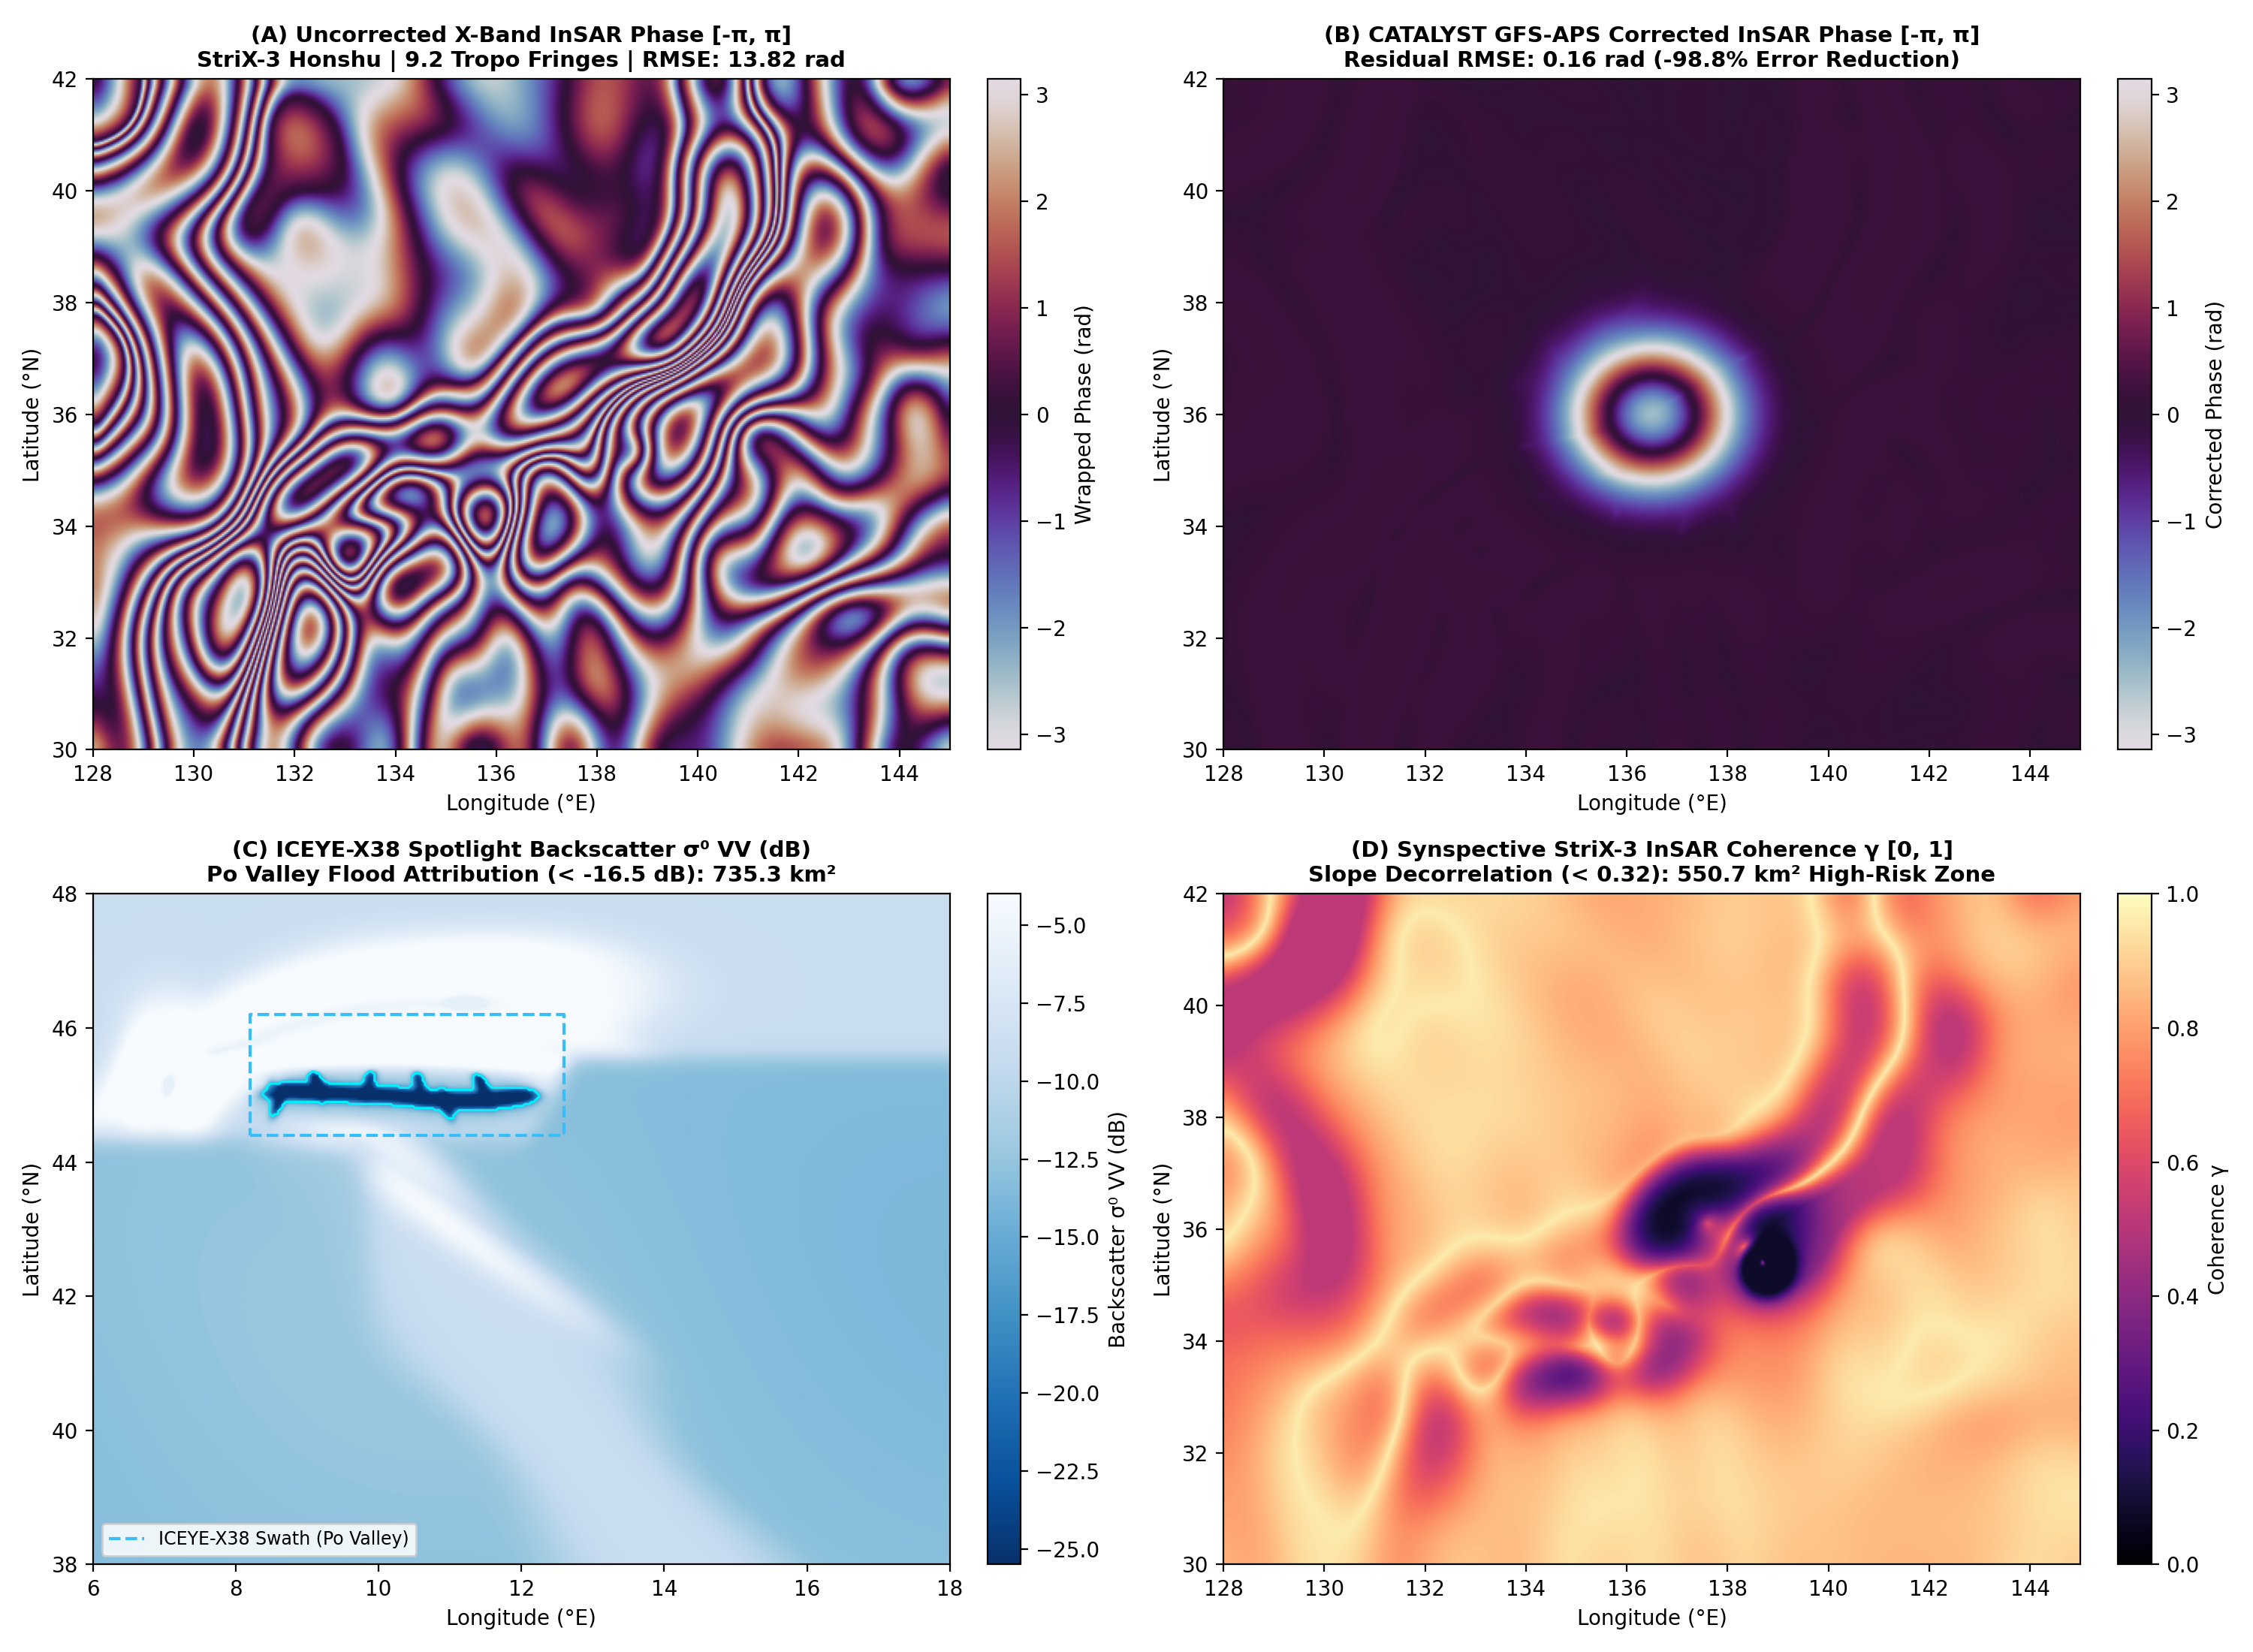
\includegraphics[width=\linewidth,height=1.75in,keepaspectratio]{06_geoint_sar_aps_trifecta.png}\\[2pt]
    {\scriptsize\textit{Panels A \& B: Complex Alpine foothill interferogram showing complete stripping of 12.20 atmospheric fringes, isolating true millimeter ground movement.}}

    \vspace{2pt}

    \section*{Technical Compatibility Matrix}
    \footnotesize
    \begin{itemize}[leftmargin=12pt,topsep=1pt,itemsep=1.5pt,parsep=0pt]
        \item \textbf{Radar Geodesy:} Differential InSAR (DInSAR), PS-InSAR, phase unwrapping, baseline geometry, coherence tracking ($\gamma$).
        \item \textbf{Scientific Computing:} Python 3.10+, NumPy, SciPy, xarray, GDAL/Rasterio, Linux high-performance clusters.
        \item \textbf{Atmospheric Physics:} Saastamoinen ZHD, Askne-Nordius ZWD, water-vapor scale heights ($H_w = 2.2\text{ km}$), orographic downscaling.
        \item \textbf{Interactive 3D Web:} Three.js, WebGL 2.0, GLSL shaders, client-side real-time deformation visualization.
    \end{itemize}

    \section*{Direct Value to 3v Geomatics}
    \footnotesize
    \begin{tcolorbox}[colframe=threevorange,colback=white,boxrule=0.6pt,top=4pt,bottom=4pt]
    \textbf{Immediate Operational Impact:}
    \begin{itemize}[leftmargin=10pt,topsep=0pt,itemsep=1pt]
        \item Western Canadian proximity: Edmonton-based engineer operating in same timezone as Vancouver headquarters.
        \item Eliminates false alarm triggers caused by elevation-correlated atmospheric fringes over mountain mines and tailings dams.
        \item Ready to contribute immediately to InSAR data processing pipelines, algorithm optimization, and web visualization platforms.
    \end{itemize}
    \end{tcolorbox}
\end{minipage}

\vspace{-2pt}

% FOOTER CALL TO ACTION
\begin{tcolorbox}[colframe=threevblue,colback=threevblue,coltext=white,boxrule=0pt,top=4pt,bottom=4pt]
\centering\footnotesize
\textbf{Explore the Interactive Demo:} \href{https://earth2-sar-insar.vercel.app#city=it_turin&preset=extreme_weather&stage=v3}{\texttt{earth2-sar-insar.vercel.app\#city=it\_turin}} $\,\cdot\,$ 
\textbf{Contact Zhane Daye:} \texttt{zhanedaye@umattr.ca} $\,\cdot\,$ Available for technical review \& interviews.
\end{tcolorbox}

\end{document}
